\documentclass{article}
\usepackage[utf8]{inputenc}
\usepackage[russian,english]{babel}
\usepackage{graphicx}
\usepackage{colortbl}
\usepackage{multicol}
\usepackage{caption}
% \usepackage{float}
\graphicspath{ {./images/} }

\newcommand{\VK}[1]{{\color{orange} {\bf (VK: #1)}}}

\title{A closer look at the impact of activation functions on Generalizability}
\author{ 
Gabriela Tsvetkova \\ 
\texttt{gabriellatsvetkova43@gmail.com} 
\and  
Under the guidance of Victor Kolev, \\ 
Stanford University
}
\date{2020}

\usepackage{biblatex}
\addbibresource{reference.bib}

\usepackage{csquotes}

\usepackage{url}
\usepackage{hyperref}
\usepackage{amsmath}
\usepackage{booktabs}
\usepackage{amsfonts}
\usepackage{amssymb}
%\usepackage{amsthm}
\usepackage{array}
\usepackage{todonotes}
%\usepackage{tabularx}
%\usepackage{natbib}
\usepackage{pgf,tikz,pgfplots}
\pgfplotsset{compat=1.15}
\usepackage{bm}
\usepackage{mathrsfs}
%\usepackage{tabulary}
\usetikzlibrary{arrows}
\usetikzlibrary[patterns]


\begin{document}

\maketitle
\begin{abstract}
 The aim of this research is to observe the impact of different activation functions on neural network's adaptiveness to unseen data. We do so by training neural networks to approximate fundamental mathematical functions and test them on data outside of the training domain. Empirically, it can be inferred that activation functions implement implicit structures in the network, which biases training towards functions similar to the behaviour of the aforementioned functions. Hence, activation functions provide an inductive bias that if properly understood can aid improve training stability and generalization.


\end{abstract}


\newpage

\renewcommand{\contentsname}{Content}

\tableofcontents

\newpage
\section{Introduction}
Over the past decades, an overwhelming body of research has been constituting the effectiveness of Deep Learning. These black-box models -- neural networks -- are not explicitly programmed for a particular task, instead an ability to optimize their performance is implemented. They do so as they gain experience starting from zero, and gradually acquire potential for recognizing certain patterns.

However, recent applications of neural networks models proved that they are very beneficial for certain tasks, but limited for others as they perform poorly on new data. Clearly, there are a few methods for improving this feature, but as observed in (Zhang et al., 2017), explicit regularization techniques scarcely contribute to it. Therefore other factors should be taken into consideration as well.

Neural networks are in essence a composition of affine transformations. However, linearity does not give the model the capacity needed to approximate any function given unlimited data and infinite time for training. That is why non-linear activation functions such as Sigmoid, Tanh, ReLU are introduced. They actively participate in the learning process so they should have some contributions to the net’s generalizability. 

As we have been experimenting with the task of approximating fundamental mathematical functions such as  $y = x^2$ and $y = x^3$, we noticed the following: it can be inferred that activation functions implement explicit structures in the network, which biases training towards functions similar to the behaviour of the aforementioned functions.

In this paper we examine the influence of 6 activation functions and provide empirical evidence for our hypothesis. This work paves way for research into the inductive biases of neural network design, which if properly exploited could improve network stability, training speed, generalization, and applicability.



\section{Concepts}
   \label{Background}
   
    \subsection{Feedforward neural network}
    A feedforward neural network consists of nodes and connections between them. Each neuron is associated with an activation and a bias and each connection -- with a certain weight.
   
    The value of the activation function of the neurons in layer $l$ is obtained by the following formula:
    
     $$\bm a^{(l)} = g(\bm W^{(l)} \bm a^{(l-1)} + \bm b^{(l)})$$
     
    Here, $n_l$ is the number of units in layer $l$; $\bm a^{(l)} \in \mathbb{R}^{n_l}$ is the vector containing the activations of the neurons in layer $l$; $\bm W^{(l)} \in \mathbb{R}^{n_l \times n_{l-1}}$ is the matrix containing the weights which connect the neurons in layer $l$ to those in layer $l-1$; $\bm b^{(l)} \in \mathbb{R}^{n_l}$ is the vector containing the biases of the neurons in layer $l$; and $g$ is some non-linear activation function.
    
   \subsection{Loss function}
    
    The loss function evaluates how well specific algorithm models the given data i.e. the error. Since we are working in a continuous domain, we use the mean square error function:
    
    $$\mathcal{L} = \frac{1}{n_L}\|\bm y - \bm a^{(L)}\|^2$$
    
    Here, $\bm y \in \mathbb{R}^{n_L}$ is the vector containing the ground truth outputs; $\bm a^{(L)} \in \mathbb{R}^{n_L}$ is the vector containing the activations of the neurons in the last layer ($L$) i.e. the vector containing the predictions; and $\|.\|$ is the Euclidean norm.   
    Two algorithms are involved in the process of learning of the neural network -- backpropagation and gradient descent. For the latter we use Adam \cite{adam} in our experiments.
    
\section{Methods}
\label{Methods}

    \subsection{Activation Functions}
    In this paper the activation functions used are as follows: \\
    \iffalse
    $$ \ \ \ \text{ReLU}(x) = \begin{cases} 
                    0 & x \leq 0 \\
                    x & x > 0 \\
                 \end{cases}$$
    
    $$\ \text{Tanh}(x) = \frac{e^x - e^{-x}}{e^x + e^{-x}}$$
    
    $$\ \ \ \ \text{SiNU}(x) = \sin(x)$$
   
    $$\ \ \ \ \text{Arctan}(x) =  \tan^{-1}(x)$$
   
    $$\ \ \ \ \text{Softplus}(x) = \ln{(1+e^{x})}$$
    
    $$\ \ \ \ \text{Swish}(x) = \frac{x}{1 + e ^ {- x}}$$
    \fi
\begin{minipage}{0.48\textwidth}
\centering
    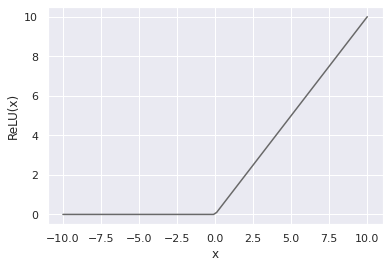
\includegraphics[width=\linewidth]{relu.png}
    \captionof{figure}{$\text{ReLU}(x) = \begin{cases} 
                    0 & x \leq 0 \\
                    x & x > 0 \\
                 \end{cases}$}
    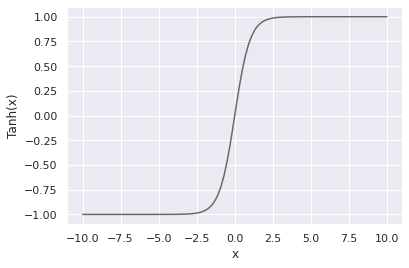
\includegraphics[width=\linewidth]{tanh.png}
    \captionof{figure}{$\text{Tanh}(x) = \frac{e^x - e^{-x}}{e^x + e^{-x}}$}
    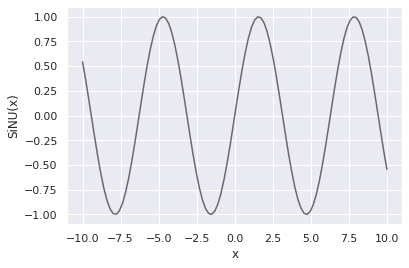
\includegraphics[width=\linewidth]{sin.png}
    \captionof{figure}{$\text{SiNU}(x) = \sin(x)$}

\end{minipage}\hspace{0.03\textwidth}%
\begin{minipage}{0.48\textwidth}
 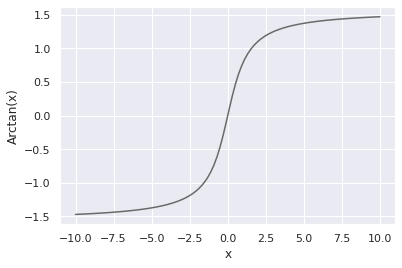
\includegraphics[width=\linewidth]{arctan.png}
    \captionof{figure}{$\text{Arctan}(x) =  \tan^{-1}(x)$\vspace{2.5em}} \par
  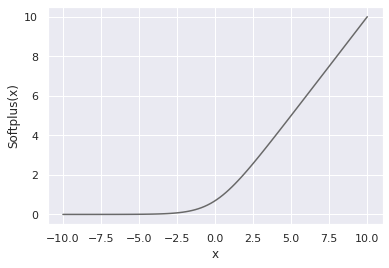
\includegraphics[width=\linewidth]{softplus.png}
    \captionof{figure}{$\text{Softplus}(x) = \ln{(1+e^{x})}$}\par
   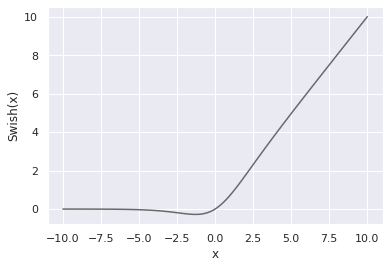
\includegraphics[width=\linewidth]{swish.png}
    \captionof{figure}{$\text{Swish}(x) = \frac{x}{1 + e ^ {- x}}$}\par
\end{minipage}
    \subsection{Spectral Norm Regularization}

Neural networks tend to learn the training examples well, but fail to generalize to new ones. This is known as overfitting, and stems from the fact that the minimum error objective is ill-posed. For instance, the Lagrange polynomial of a set of points would have the smallest loss, yet it would not have high generalization error.

One method of alleviating overfitting is regularization. This is the process of penalizing big values in the weight matrix with the effect of deriving a model which adapts well to new data
  
In this work we focus on spectral norm regularization\cite{spectral}. 
It is explicitly shown that this method contributes the most to the generalizability of the model from other existing methods such as Weight Decay, Dropout, Jacobian regularization, just to name a few. (Neyshaubar etal 2019)\cite{Neyshaubar} and \cite{Arora}. The general idea behind it is to make the model insensitive to small input perturbation, which is central for its adaptiveness to new examples. This is achieved by using the spectral norm or in other words, the largest single value of a matrix \boldsymbol{W} $ \in \mathbb{R}^ {m\times n} $:
$$\sigma = \max_{\xi \in \mathbb{R}^ {n}, \xi \neq 0}\dfrac{ \|A\xi\|_2}{\|\xi\|_2}$$

Then for a small perturbation $\boldsymbol{\xi} \in \mathbb{R}$ where $f_\theta$ is the objective function and $\boldsymbol{W}_{\Theta,x} \in \mathbb{R}^{n_0\times n_L}$, $\boldsymbol{b}_{\Theta, x} \in \mathbb{R}^{n_L}$ are weight matrix and bias vector respectively:

\begin{equation*}
    \begin{split}
        \frac{\left\|f_{\Theta}(\boldsymbol{x}+\boldsymbol{\xi})-f(\boldsymbol{x})\right\|_{2}}{\|\boldsymbol{\xi}\|_{2}}&=\frac{\left\|\left(W_{\Theta, \boldsymbol{x}}(\boldsymbol{x}+\boldsymbol{\xi})+\boldsymbol{b}_{\Theta, \boldsymbol{x}}\right)-\left(W_{\Theta, \boldsymbol{x}} \boldsymbol{x}+\boldsymbol{b}_{\Theta, \boldsymbol{x}}\right)\right\|_{2}}{\|\boldsymbol{\xi}\|_{2}}=\\
        &=\frac{\left\|W_{\Theta, x} \boldsymbol{\xi}\right\|_{2}}{\|\boldsymbol{\xi}\|_{2}} \leq \sigma\left(W_{\Theta, \boldsymbol{x}}\right)
    \end{split}
\end{equation*}

$$$$

\subsection{Approach}

Our approach is to train a neural model to approximate $y=x^{2}$ or $y=x^{3}$ only with the help of spectral norm regularization on the interval $[-15;15]$. Then we see how the model generalize on the interval $[-40;40]$. All the networks have a dense-layered architecture and the maximum units of a layer $L$ are no more than 256.







\section{Results}
\label{Results}
 
In the graphs below are illustrated the models with the best performance on the two tasks.

\begin{figure*}[H]
\begin{multicols}{2}
    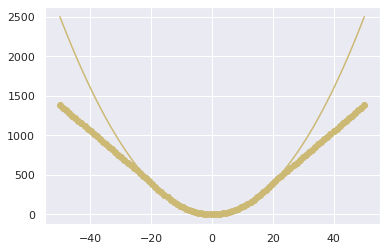
\includegraphics[width=\linewidth]{ReLUx2.png}\par 
    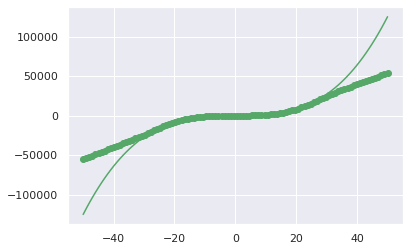
\includegraphics[width=\linewidth]{ReLUx3.png}\par 
\end{multicols}
\caption{The left graph shows a model that approximates $y = x^2$ trained on range [-15;15] with ReLU. It is visible that the graph of the objective function keeps a linear structure because of its activation function. The same can be inferred for the right graph of $y=x^3$. }
\begin{multicols}{2}
    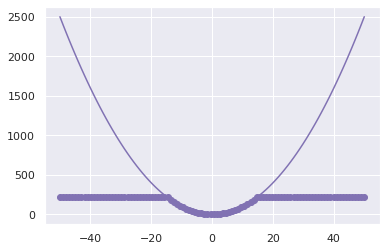
\includegraphics[width=\linewidth]{Tanhx2.png}\par
    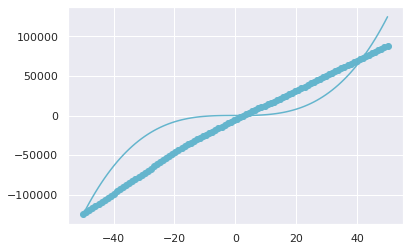
\includegraphics[width=\linewidth]{Tanhx3.png}\par
\end{multicols}
\caption{The left graph shows a model that approximates $y = x^2$ trained on range [-15;15] with Tanh. It is visible that the graph of the objective function keeps a linear structure because of its activation function. The same can be inferred for the right graph of $y=x^3$.}
\end{figure*}
\begin{figure*}[H]
\begin{multicols}{2}
    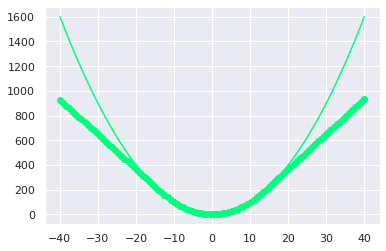
\includegraphics[width=\linewidth]{arctan2.png}\par
    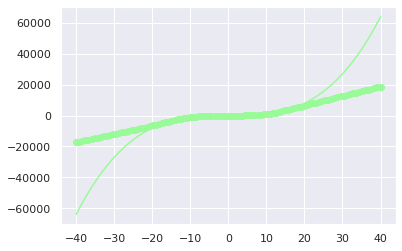
\includegraphics[width=\linewidth]{arctan3.png}\par
\end{multicols}
\caption{The left graph shows a model that approximates $y = x^2$ trained on range [-15;15] with Arctan. It is visible that the graph of the objective function keeps a linear structure because of its activation function. The same can be inferred for the right graph of $y=x^3$.}
\end{figure*}

\begin{figure*}[H]
\begin{multicols}{2}
    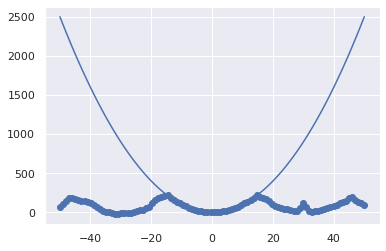
\includegraphics[width=\linewidth]{x2_SiNU.png}\par
    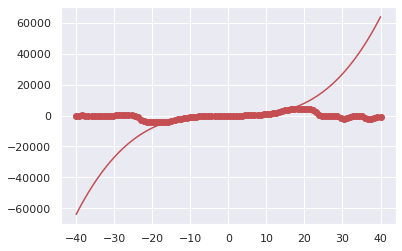
\includegraphics[width=\linewidth]{x3_SiNU.png}\par
\end{multicols}
\caption{The left graph shows a model that approximates $y = x^2$ trained on range [-15;15] with SiNU. It is visible that the graph of the objective function keeps a sinusoidal structure because of its activation function. The same can be inferred for the right graph of $y=x^3$.}
\end{figure*}
\begin{figure*}[H]
\begin{multicols}{2}
    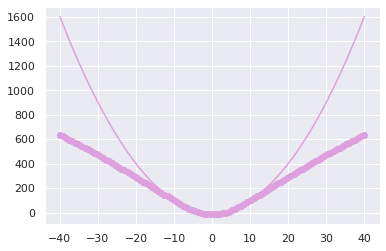
\includegraphics[width=\linewidth]{swish2.png}\par
    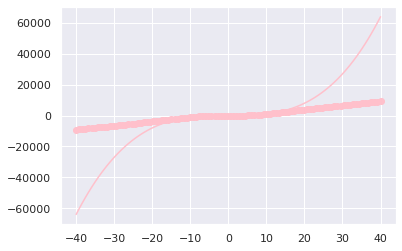
\includegraphics[width=\linewidth]{swish3.png}\par
\end{multicols}
\caption{The left graph shows a model that approximates $y = x^2$ trained on range [-15;15] with Swish. It is visible that the graph of the objective function keeps a linear structure because of its activation function. The same can be inferred for the right graph of $y=x^3$.}
\end{figure*}
\begin{figure*}[H]
\begin{multicols}{2}
    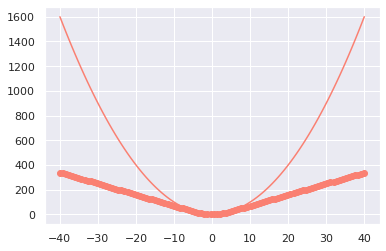
\includegraphics[width=\linewidth]{softplus2.png}\par
    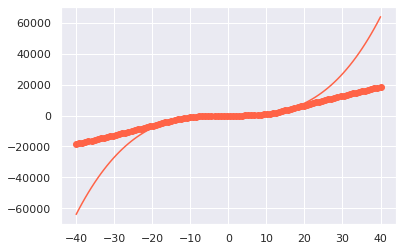
\includegraphics[width=\linewidth]{softplus3.png}\par
\end{multicols}
\caption{The left graph shows a model that approximates $y = x^2$ trained on range [-15;15] with Softplus. It is visible that the graph of the objective function keeps a linear structure because of its activation function. The same can be inferred for the right graph of $y=x^3$.}
\end{figure*}
\newpage



\section{Future Development}
\label{Future Work}
Experiments such as changing the range of input data, type of function, the architecture of the neural network and the type of regularization Dropout\cite{dropout} are always interesting and may lead to better understanding of the impact of activation functions.
A further investigation with modular neural networks \cite{gnn} for composing complex functions can be made.


\section{Conclusion}
\label{Conclusion}
In the present work, we showed empirically that the choice of activation functions has an impact on what the neural network learns, and it provides a strong bias, especially in points outside of the training domain. Such an inductive bias may be exploited by machine learning engineers to ease training, improve stability and aid generalization performance by embedding implicit structure in the network. 



\printbibliography
\end{document}